\chapter{The Sub-Problem Structure of Manipulation Tasks}
\label{chap:formulation}

In this chapter,
we lay out the structure of the manipulation planning problem.

Definitely reference DRC Trials paper for planning vs. execution
time breakdown!

We are NOT solving the symbolic task planning problem.
Our pieces would be useable by such a planner,
including one which reasons about different orders.
But for the purpose of this thesis,
we'll basically assume that the sequence is given to us.

\section{Sub-Problem Structure}

{
\setlength{\offsetpage}{0.5in}
\begin{figure}
\begin{widepage}
\centering

   \begin{subfigure}[t]{0.19\linewidth}
      \centering
      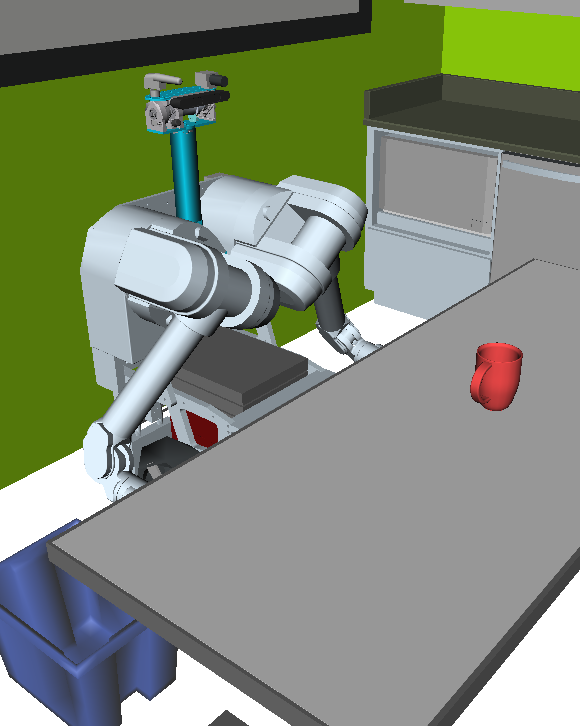
\includegraphics[width=\columnwidth]{figs/testherb-a.png}
      \caption{Start config}
   \end{subfigure}
   \begin{subfigure}[t]{0.19\linewidth}
      \centering
      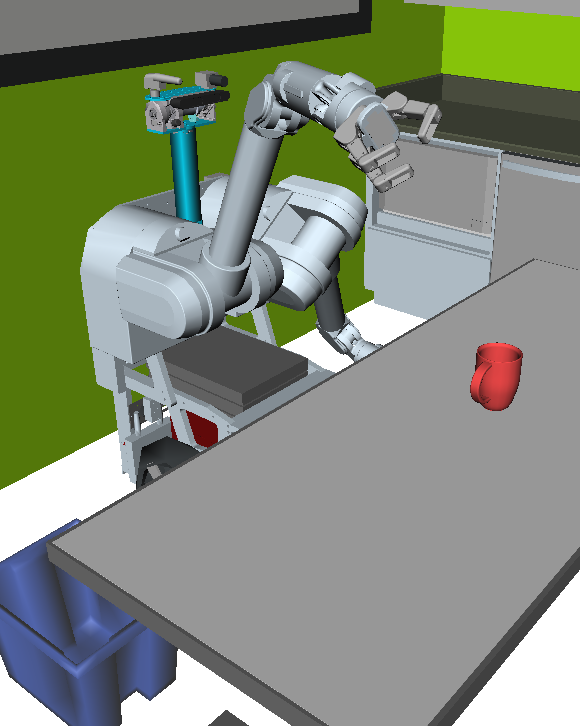
\includegraphics[width=\columnwidth]{figs/testherb-b.png}
      \caption{Step 1 in $X_1$}
   \end{subfigure}
   \begin{subfigure}[t]{0.19\linewidth}
      \centering
      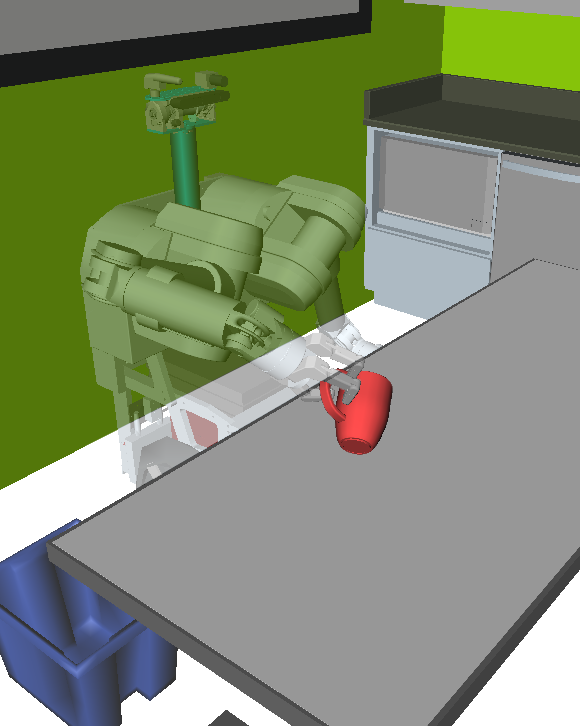
\includegraphics[width=\columnwidth]{figs/testherb-c.png}
      \caption{Step 2 in $X_2$}
   \end{subfigure}
   \begin{subfigure}[t]{0.19\linewidth}
      \centering
      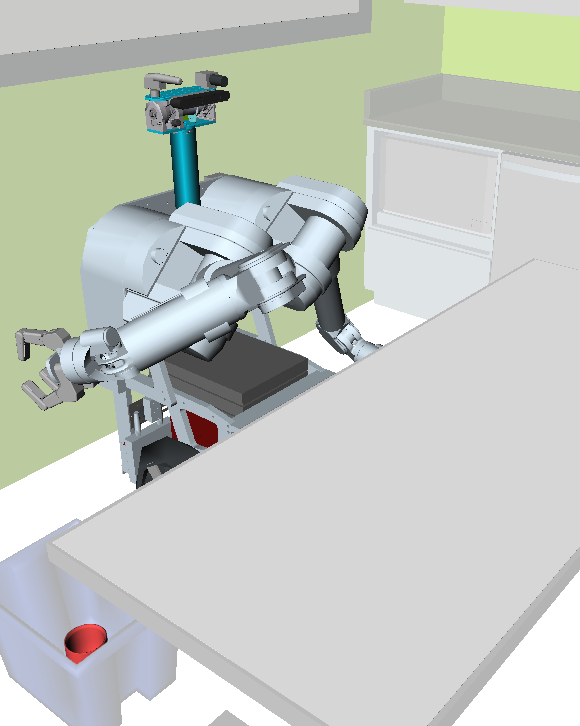
\includegraphics[width=\columnwidth]{figs/testherb-d.png}
      \caption{Step 3 in $X_3$}
   \end{subfigure}
   \begin{subfigure}[t]{0.19\linewidth}
      \centering
      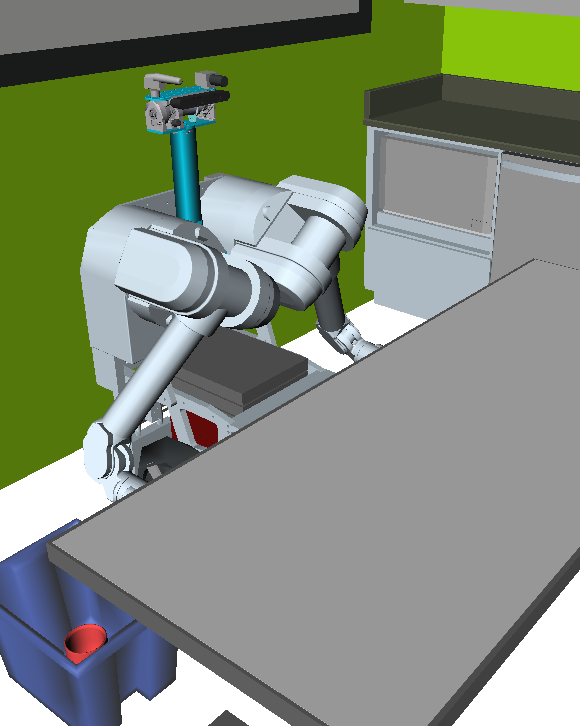
\includegraphics[width=\columnwidth]{figs/testherb-e.png}
      \caption{End config}
   \end{subfigure}

   \vspace{0.3cm}

   \begin{subfigure}[t]{\linewidth}
      \centering
      \includegraphics{build/diagram-multi-step}
      \caption{This thesis focuses on efficient geometric planning
         for manipulation tasks (the lower two levels here).
         Task planning can be performed by an autonomous
         symbolic planner,
         or guided by a human operator.}
   \end{subfigure}

   \caption{Diagram of multi-step planning framework.}
   \label{fig:diagram-multi-step}
\end{widepage}
\end{figure}
}

The manipulation problem has a particular structure,
which we discuss here.
See Figure~\ref{fig:diagram-multi-step}
for a diagram.

Briefly discuss the higher-level planner.
Not doing research here -- just need something that specifies
geometric goals.
Complementary to symbolic planners
or from humans (e.g. the DRC \cite{dellin2014drc}).
For this proposal,
will only discuss seqential sub-plans,
but an intelligent meta-planner
can do non-sequential stuff too.

\section{Motivation: DRC Trials}

Talk a lot about the DRC approach.
It was slow, and it got stuck!

Copy-paste in from the ISER paper!

\section{Multi-Step Approach}

Multi-step problem structure (lots of options at each step);
decomposition into a bunch of "local planner" like things.
We're essentially building a meta-graph.
Don't get stuck.

We talk a lot about the mapping
from continuous spaces to graphs in
Chapter~\ref{chap:graphs-in-continuous}.

Talk about subgoals in A* literature.

For now, assume a prescribed order,
but we'll talk later about more complex meta-planning
approaches.

\section{DRC Trials Approach}

Used a bidirectional RRT.
Deep-dive into DRC Trials data analysis from ISER paper.

\section{Root Sampling}

Do sampling at this higher level.
(Can't rely on the sub-planners to generate their own starts/goals --
they must be synchronized.)
Potential research question: learn good intermediate goals.

\subsection{Two Ways to Make it Fast}

The proposal is split into two complementary things,
guided by how slow collision checking is.

Chapters 3,4 focus WITHIN each step.
Make each step fast.

Chapters 5,6 focus BETWEEN steps.
Exploit structure between steps (Chapter~\ref{chap:multi-set}).
Single-query vs. multi-query.

\section{Within-Step Approach}

While there are many types of approaches for such queries
which we discuss in Section~\ref{sec:related-work},
one of the most common are graph search algorithms.

\paragraph{General Problem Characterization.}

We are motivated to solve motion planning problems for articulated robots.
In the simplest version of this problem,
the robot has a continuous configuration space $C$,
with some subset $C_{obs}$ in collision.
All feasible trajectories must then lie entirely in
$\mathcal{C}_{\mbox{\scriptsize free}} = C \setminus C_{obs}$.
In general, testing some configuration $q$ for membership in
$\mathcal{C}_{\mbox{\scriptsize free}}$
is an expensive operation.
A typical query asks for a trajectory $t: [0,1] \rightarrow Q$ between
a start set and a goal set (e.g. $t(0) \in Q_s$ and $t(1) \in Q_g$.
We defer discussion constraints until later.
We are focused on configuration spaces without dynamics.

In this chapter,
we'll primarly focus on single-query things,
but we'll keep in mind that we want things that can enable reuse eventually.

\section{Related Work}

While we will primarily apply graph search techniques to this problem,
we start by reviewing alternative approaches.

\section{Review of Alternative Approaches}
\label{sec:related-work}

Since $C$ is continuous,
all approaches must introduce some sort of discretization
in order to compute solutions.
We choose to build a graph consisting of vertices and edges in $C$,
and then search that graph (Section~\ref{sec:best-first}).
We do this because we can rely on existing techniques,
and because an explicit graph can be more easily reused than other
approaches.
In this section, we discuss alternative approaches to solving
the motion planning problem for articulated robots.

%\subsection{Multi-Query Approaches}
%
%We could run a PRM \cite{kavrakietal1996prm}.
%Commit to a fixed graph,
%and determine the validity of each vertex and edge w.r.t.
%$\mathcal{C}_{\mbox{\scriptsize free}}$.
%Then, at query time,
%run A* to find the shortest path (this is fast due to graph sparseness).
%This is good because it reuses work.
%Unfortunately,
%(a) our $\mathcal{C}_{\mbox{\scriptsize free}}$
%is different for every subplan
%(and for different options with each),
%and (b) we don't want to determine validity over the entire graph
%because it's costly.

\subsection{Anytime algorithms}

Compare to RRT*, FMT*, BIT*, etc.

\subsection{Other}

Need to look into the SBL planner \cite{sanchezante2001sbl}
(Single Query BiDirectional Lazy PRM).

\subsection{Incremental Construction Algorithms}

We could construct the graph incrementally and in response to the shape
of $\mathcal{C}_{\mbox{\scriptsize free}}$.
RRTs behave well for quickly finding feasible paths.
We'll compare against them at the end of this chapter.
Also talk about ESTs.
Difficult to cache things.

\subsection{Trajectory Optimization}

One approach is trajectory optimization.
For example, there's CHOMP \cite{zucker2013chomp}
and TrajOpt \cite{schulman2013trajopt}.
Lots of other prior work here that is not manipulation-focused.

Local minima problems.
Difficult to cache / apply to similar problems.

This is largely complementary.
Use sampling-based planning to quickly find feasible solutions,
and then optimize them.

\section{Other Stuff}

Other stuff to touch on:
\begin{itemize}
\item Dealing with constraints
\item Dealing with dual-arm stuff
\item Dealing with optimizers (run afterwards!)
   Most solution paths will be unexecuted, so optimize later!
\end{itemize}
